\clearpage
\section{Results}
\label{tW_Results}

\textbf{Note:} before going to measure the limit on EFT couplings, it is worth to mention that a cross check on measuring SM tW cross section is performed (see appendix \ref{App_tW_XS}) which makes sure we have understand the SM tW part.

\medskip

In order to calculate the total cross sections for the t$\bar{\rm t}$ and tW processes and generate events in the presence of new effective interactions, we implement the operators of equations \ref{eq1}~in the universal FeynRules output format \cite{Degrande:2011ua} through the
Feynrules package \cite{Alloul:2013bka} and use the {\sc MadGraph5\_}a{\sc mc@NLO} event generator~\cite{MADGRAPH,Alwall:2014hca} at the leading order (LO).
If we allow for the presence of one operator at a time, the total cross section up to $\mathcal{O}(\Lambda^{-4})$ can be parameterised as

\begin{equation}
\label{eq:Limit}
        \sigma=\sigma_{SM}+
        C_i\sigma_i^{(1)}+
    C_i^2\sigma_{i}^{(2)}\,,
\end{equation}

where the $C_i$'s are effective  couplings introduced in equations \ref{eq1}. Here, $\sigma_i^{(1)}$ is the cross section of the interference term between the SM diagrams. The cross section $\sigma_i^{(2)}$ is the pure new physics contribution.
We use the most precise available SM predictions for $\sigma_{\text{SM}}$, which are $\sigma_{SM}^{t\bar{t}} = 832^{+20}_{-29}(scales)\pm 35(PDF+\alpha_{s})pb$ and $\sigma_{SM}^{tW} = 71.7^{+1.8}_{-1.8}(scales)\pm 3.4(PDF+\alpha_{s})pb$ for \ttbar~ and tW production, respectively \cite{Czakon:2011xx,Kidonakis:2015nna}.
The scales reflects uncertainties  in  the  factorization and  renormalization scales.
In the framework of EFT, the $\sigma_i^{(1)}$  and $\sigma_i^{(2)}$ terms are calculated at NLO accuracy for all of the operators except $O_G$.
The values of $\sigma_i^{(1)}$ and $\sigma_i^{(2)}$ for various effective couplings at LO and available K-factors are given in Table \ref{xsVScoupling}.



\begin{table}[h]
\caption{Cross sections for \ttbar~ and tW production [in pb] for the various effective couplings for $\Lambda$  = 1 TeV. The respective available K-factors are also shown.
}
\label{xsVScoupling}
\centering
\begin{tabular}{|l|l|l|l|l|l|l|l|}
\hline
Channel & Variable & $C_{G}$ & $C_{\phi q}^{(3)}$ & $C_{tW}$ & $C_{tG}$ & $C_{uG}$ & $C_{cG}$   \\
\hline
\hline
\multirow{4}{*}{\ttbar} &   $\sigma_i^{(1)-LO}$  &  31.9    & -   & -   & 137    & -   & -             \\
 &   $\sigma_i^{(1)-NLO}/\sigma_i^{(1)-LO}$  &  -   & -   & -   & 1.48 \cite{Franzosi:2015osa} & -   & -             \\
 &   $\sigma_i^{(2)-LO}$  &  102.3   & -   & -   & 16.4    & -   & -             \\
 &   $\sigma_i^{(2)-NLO}/\sigma_i^{(2)-LO}$  &  -   & -   & -   & 1.44 \cite{Franzosi:2015osa}  & -   & -             \\
 \hline
 \hline
\multirow{4}{*}{tW} &   $\sigma_i^{(1)-LO}$  &  -   & 6.7   & $-$4.5    & 3.3   & 0  & 0             \\
 &   $\sigma_i^{(1)-NLO}/\sigma_i^{(1)-LO}$ &  -   & 1.32  \cite{Zhang:2016omx}   & 1.27 \cite{Zhang:2016omx}  & 1.27 \cite{Zhang:2016omx}   & 0   & 0             \\
 &   $\sigma_i^{(2)-LO}$  &  -   & 0.2   & 1    & 1.2   & 16.2   & 4.6             \\
 &   $\sigma_i^{(2)-NLO}/\sigma_i^{(2)-LO}$ &  -   & 1.31 \cite{Zhang:2016omx}   & 1.18 \cite{Zhang:2016omx}   & 1.06 \cite{Zhang:2016omx}  & 1.27 \cite{Durieux:2014xla}  &1.27 \cite{Durieux:2014xla} \\
 \hline
\end{tabular}
\end{table}


\subsection {Limit setting procedure}
\label{tW_limit_set}
For those operators which interfere with the SM, C$_{G}$-C$_{tG}$-C$_{\phi q}$-C$_{tW}$, normalization of the \ttbar~ or tW process is directly extracted from a fit to data.
Normalization of the signal (tW/ \ttbar) is parameterized using equation \ref{eq:Limit} in which $\sigma_{SM}$, $\sigma_i^{(1)}$ and $\sigma_{i}^{(2)}$ are fixed parameters (see Table \ref{xsVScoupling}) and C is the parameter of interest in the fit.
In order to evaluate the effect of the uncertainties on $\sigma_{SM}$, $\sigma_i^{(1)}$ and $\sigma_{i}^{(2)}$, fit is performed when these parameters are varied $\pm\sigma$ because of the Q scale uncertainties.
All three terms are considered fully correlated for Q-scale variation based on the recommendation from theorists.
In addition, uncertainties due to PDF is considered. Results of the mentioned variations are only shown for observed limits for comparison to the nominal results.
In Table \ref{xspunc}, nominal values for $\sigma_i^{(1)}$ and $\sigma_{i}^{(2)}$ are shown together with errors.

\begin{table}[h]
\caption{Cross sections for \ttbar~ and tW production [in pb] for the various effective couplings for $\Lambda$  = 1 TeV together with Q-scale errors.
}
\label{xspunc}
\centering
\scalebox{0.7}{
\begin{tabular}{|l|l|}
\hline
Channel               & $\sigma_{SM}$ (scale unc.) (PDF+alphaS unc.)                                                       \\ \hline
\ttbar                & 831.76 (+19.77, -29.20), (+35.06, -35.06)                                                          \\ \hline
tW                    & 71.7 (+1.80, -1.80), (+3.40 -3.40)                                                                 \\ \hline  \hline
Channel               &$\sigma_i^{(1)}$ (scale unc.)                                                                         \\ \hline
\ttbar                & 202.83 $C_{tG}$ (+24.54,-26.98) , 31.9 $C_{G}$ (+8.1,-6.9)                                                              \\ \hline
tW                    & 8.844 $C_{\phi q}$ (+0,-0) ,-5.65 $C_{tW}$ (+0.08317,-0.061846) , 4.223 $C_{tG}$ (+0.0294,-0.0398)                                     \\ \hline  \hline
Channel               & $\sigma_i^{(2)}$ (scale unc.)                                                                        \\ \hline
\ttbar                & 23.545 $C_{tG}^2$ (+0,-0) , 102.3 $C_{G}^2$ (+22.7,-15.3) \\ \hline
tW                    & 0.275 $C_{\phi q}^2$ (+0,-0) , 1.18 $C_{tW}^2$ (+0.0283,-0.0257) , 1.322 $C_{tG}^2$ (+0.0558,-0.0335) , 21.209 $C_{uG}^2$ (+1.485,-1.273) , 5.804 $C_{cG}^2$ (+0.255,-0.250) \\ \hline  \hline
\end{tabular}}
\end{table}

\textbf{Note:} Before going the limit result it is worth mention that all these studies are also performed using $e\mu$ final states. Therefore results from $e\mu$ channel are shown for comparison and the results for ee, $e\mu$ and $\mu\mu$ channels combined are also shown.

\subsection {Exclusion limits on \texorpdfstring{C$_{G}$ effective coupling}{}}

It was discussed in Section \ref{tW_Int} that the operator $O_{G}$ operator only contributes to \ttbar~ production process.
It was found that the shapes of some variables are affected in the presence of the $O_{G}$ operator.
On the other hand, the effect is not  big enough to be observed experimentally in \ttbar~ kinematic distributions as a shape effect.
Therefore, the fit is  performed simultaneously on the observed event yield in  (1-jet,1-tag), (2-jet,1-tag) and ($\geq$2-jet,2-tag) categories for ee and $\mu\mu$ channels.
The results for ee, $\mu\mu$ and $e\mu$ individual channels and combined channels are listed in  Table \ref{tab:EFT_Limit_CG}.
The results of the combined likelihood scans of the C$_{G}$ coupling is shown in Figure \ref{fig:EFT_scan_CG}.


\begin{table}[h]
\centering
\scalebox{0.8}{
\begin{tabular}{|l|l|l|l|l|}
\hline
                              &               Regions            & best fit exp./obs. & 68\% exp./obs.limit                    & 95\% exp./obs.limit   \\ \hline                                                  \multirow{4}{*}{$C_{G}$}   & ee       yield (1j1t), (2j1t), ($\geq$2j,2t)          & 0.00 / -0.14       &{[}-0.90 to 0.59{]}/{[}-0.82 to 0.51 {]}& {[}-1.20 to 0.88{]}/{[}-1.14 to 0.83{]} \\ \cline{2-4}
                              & $\mu\mu$ yield (1j1t), (2j1t), ($\geq$2j,2t)          & 0.00 / -0.14       &{[}-0.88 to 0.57{]}/{[}-0.75 to 0.44 {]}& {[}-1.16 to 0.85{]}/{[}-1.06 to 0.75{]} \\ \cline{2-4}
                              & e$\mu$   yield (1j0t), (1j1t), (2j1t), ($\geq$2j,2t)  & 0.00 / -0.18       &{[}-0.82 to 0.51{]}/{[}-0.73 to 0.42 {]}& {[}-1.08 to 0.77{]}/{[}-1.01 to 0.70{]} \\ \cline{2-4}
                              & Combined                                              & 0.00 / -0.18       &{[}-0.82 to 0.51{]}/{[}-0.73 to 0.42 {]}& {[}-1.07 to 0.76{]}/{[}-1.01 to 0.70{]} \\ \hline \hline
\end{tabular}}
\caption{Summary of allowed 68\% CL and 95\% CL intervals on C$_{G}$ effective coupling  obtained in $ee$, $e\mu$, $\mu\mu$ and combined channels ($\Lambda = 1 TeV$).}
\label{tab:EFT_Limit_CG}
\end{table}

\begin{figure}[ht]
  \begin{center}
      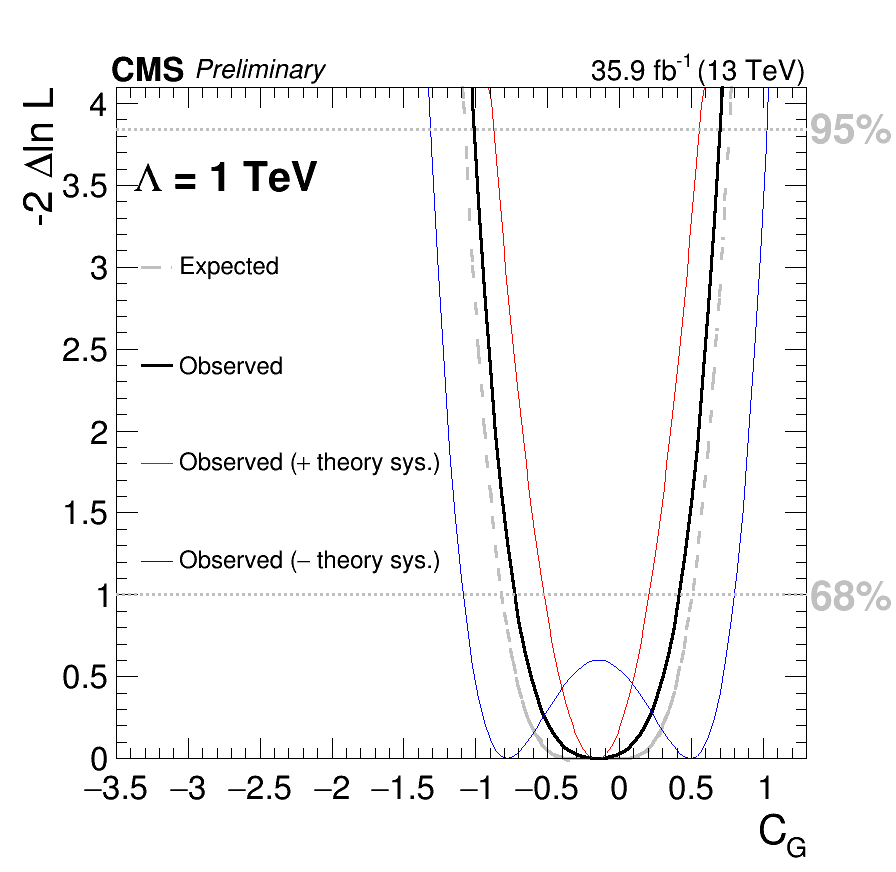
\includegraphics[width=0.45\textwidth]{figures/tW/fig/scan_all_plot/Cg_combined_scan.png}
    \caption{Likelihood scan of C$_{G}$ effective coupling for combined channels.
    \label{fig:EFT_scan_CG}}
  \end{center}
\end{figure}

\clearpage
\subsection {Exclusion limits on \texorpdfstring{C$_{tG}$, C$_{\phi q}$ and C$_{tW}$ effective couplings}{}}
The deviation from the SM tW production from the interference terms between the
SM and the $O_{tG}$, $O_{\phi q}$ and $O_{tW}$ operators is of the order of $\frac{1}{\Lambda^2}$.
It is assumed that the new physics scale, $\Lambda$, is larger  than the scale we  probe. Therefore, $\frac{1}{\Lambda^4}$
contributions, pure new physics term, would be small compared to the contribution from the interference term.
Following the strategy described in Section \ref{tW_limit_set}, in the likelihood fit, the signal probability density function (pdf) originates from the sum of the SM term, the interference term and the pure new physics term is assumed to be the same as the SM tW (or \ttbar~ for $O_{tG}$) pdf.


In order to set limits on the effective couplings $C_{tG}$, $C_{\phi q}$ and $C_{tW}$, we utilize the MLP output distributions for both data and MC expectation in the (1jet,1b-jet)
and (2jet,1b-jet) regions and event yield in the ($\geq$2jet,2b-jet) region for ee and $\mu\mu$ channels.
The MLP is trained to separate tW from \ttbar~ events as was discussed in Section \ref{signal}.
The inclusion of the ($\geq$2jet,2b-jet) and (2jet,1b-jet) regions helps to constrain the normalization and systematic uncertainties of the \ttbar~ background.
Comparison between observed data and the SM background prediction for the MLP output shape in various jet-bjet regions are shown in Figure \ref{fig:limit_binee}.


\begin{figure}[ht]
  \begin{center}
    \begin{tabular}{ccc}
      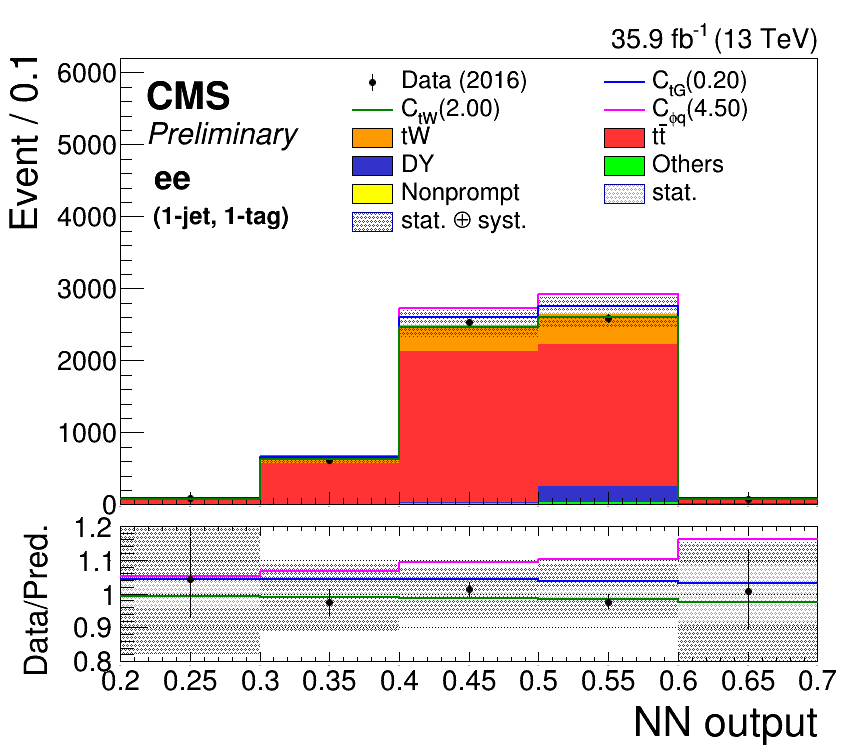
\includegraphics[width=0.45\textwidth]{figures/tW/fig/Result/ee/H_MLP_1jet_1bjet.png} &
      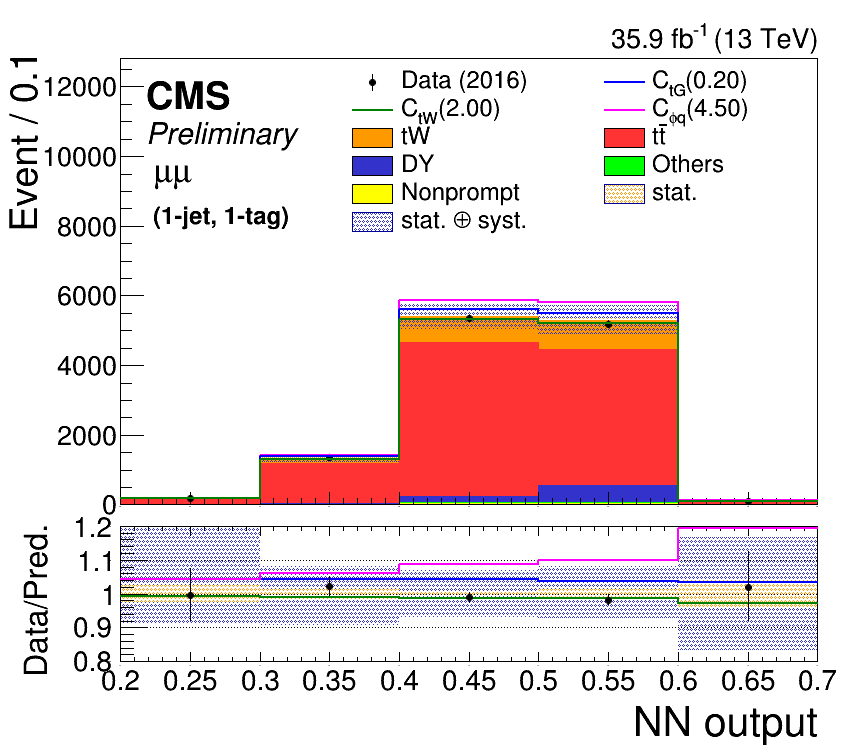
\includegraphics[width=0.45\textwidth]{figures/tW/fig/Result/mumu/H_MLP_1jet_1bjet.png}\\
      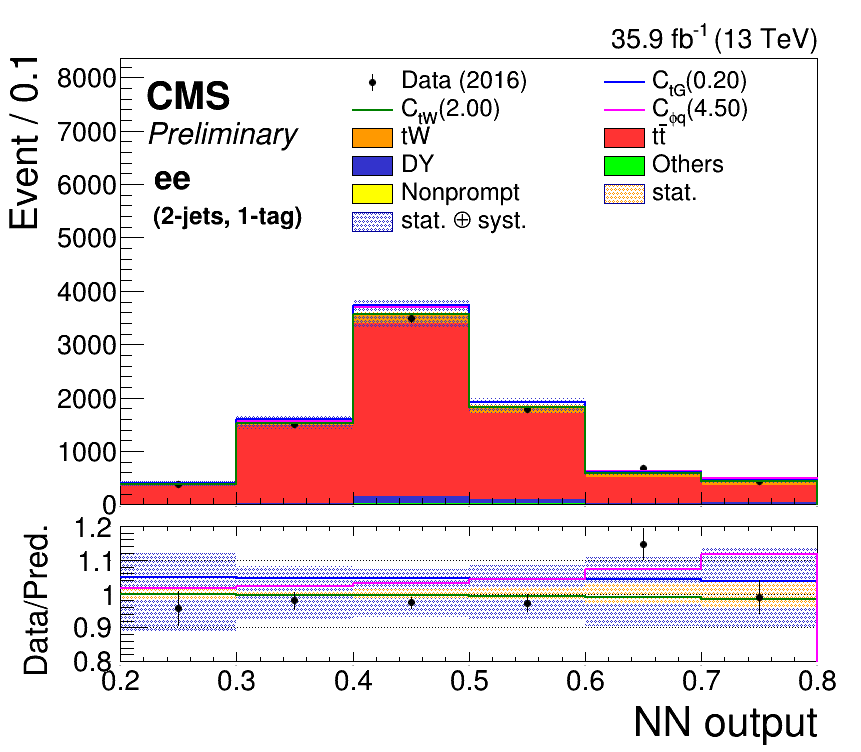
\includegraphics[width=0.45\textwidth]{figures/tW/fig/Result/ee/H_MLP_2jet_1bjet.png} &
      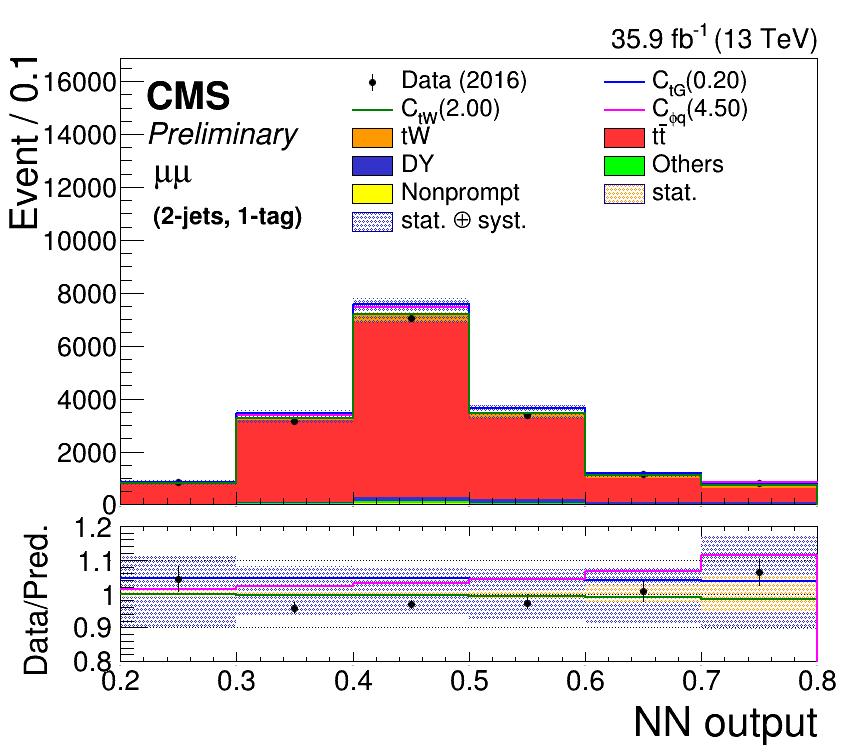
\includegraphics[width=0.45\textwidth]{figures/tW/fig/Result/mumu/H_MLP_2jet_1bjet.png}\\
    \end{tabular}
    \caption{The MLP distribution of data and MC in different regions: (1jet,1b-jet) (top row), (2jet,1b-jet) (bottom row) used in limit setting for $ee$ channel (left column) and $\mu\mu$ channel (right column). The blue hatched bands correspond to the sum of statistical and systematic uncertainties in the event yield for the sum of signal and background predictions. The ratios of data to the sum of the predicted yields are shown at the bottom of each plot. Here, an additional solid yellow band represents the contribution from the statistical uncertainty in the MC simulation.
    \label{fig:limit_binee}}
  \end{center}
\end{figure}


Three Wilson coefficients sensitive to new physics contribution in top quark interactions, as defined in in equations \ref{eq1} are tested in observed data.
The results for individual channels and combined channels are listed in Table \ref{tab:EFT_Limit}.
The results of the combined likelihood scans of the Wilson coefficients on the full 13 TeV dataset are shown in Figure \ref{fig:EFT_scan} for  combined channels.



\begin{table}[h]
\centering
\scalebox{0.75}{
\begin{tabular}{|l|l|l|l|l|}
\hline
                              &                                                              & best fit exp./obs. & 68\% exp./obs.limit                    & 95\% exp./obs.limit   \\ \hline
\multirow{4}{*}{$C_{\phi q}$} & ee       NN output for (1j1t+2j1t) + yields($\geq$2j,2t)     & 0.00 / 1.12  &{[}-2.53 to 1.74{]}/{[}-1.18 to 2.89 {]}& {[}-6.40 to 3.27{]}/{[}-4.03 to 4.37{]}\\\cline{2-4}
                              & $\mu\mu$ NN output for (1j1t+2j1t) + yields($\geq$2j,2t)     & 0.00 / 1.13  &{[}-2.20 to 1.92{]}/{[}-0.87 to 2.86 {]}& {[}-4.68 to 3.66{]}/{[}-3.58 to 4.46{]}\\\cline{2-4}
                              & e$\mu$   NN output for (1j0t+1j1t+2j1t) + yields($\geq$2j,2t)& 0.00 / -0.70 &{[}-1.34 to 1.12{]}/{[}-2.16 to 0.59 {]}& {[}-2.57 to 2.15{]}/{[}-3.74 to 1.61{]}\\\cline{2-4}
                              &       Combined                                               & 0.00 / -1.52 &{[}-1.05 to 0.88{]}/{[}-2.71 to -0.33{]}& {[}-2.04 to 1.63{]}/{[}-3.82 to 0.63{]}\\\hline \hline
\multirow{4}{*}{$C_{tW}$}     & ee       NN output for (1j1t+2j1t)+yields($\geq$2j,2t)       & 0.00 / 6.18  &{[}-2.02 to 6.81{]}/{[}-3.02 to 7.81 {]}& {[}-3.33 to 8.12{]}/{[}-4.16 to 8.95{]}\\\cline{2-4}
                              & $\mu\mu$ NN output for (1j1t+2j1t)+yields($\geq$2j,2t)       & 0.00 / -1.40 &{[}-2.18 to 6.97{]}/{[}-3.00 to 7.79 {]}& {[}-3.63 to 8.42{]}/{[}-4.23 to 9.01{]}\\\cline{2-4}
                              & e$\mu$   NN output for (1j0t+1j1t+2j1t)+yields($\geq$2j,2t)  & 0.00 / 1.64  &{[}-1.40 to 6.19{]}/{[}-0.80 to 5.59 {]}& {[}-2.39 to 7.18{]}/{[}-1.89 to 6.68{]}\\\cline{2-4}
                              & Combined                                                     & 0.00 / 2.38  &{[}-1.14 to 5.93{]}/{[}0.22 to 4.57  {]}& {[}-1.91 to 6.70{]}/{[}-0.96 to 5.74{]}\\\hline \hline
\multirow{4}{*}{$C_{tG}$}     & ee     NN output for (1j1t+2j1t)+yields($\geq$2j,2t)         & 0.00 / -0.19 &{[}-0.22 to 0.21{]}/{[}-0.40 to 0.02 {]}& {[}-0.44 to 0.41{]}/{[}-0.65 to 0.22{]}\\\cline{2-4}
                              & $\mu\mu$ NN output for (1j1t+2j1t)+yields($\geq$2j,2t)       & 0.00 / -0.15 &{[}-0.19 to 0.18{]}/{[}-0.34 to 0.02 {]}& {[}-0.40 to 0.35{]}/{[}-0.53 to 0.19{]}\\\cline{2-4}
                              & e$\mu$   NN output for (1j0t+1j1t+2j1t)+yields($\geq$2j,2t)  & 0.00 / -0.03 &{[}-0.17 to 0.15{]}/{[}-0.19 to 0.11 {]}& {[}-0.34 to 0.29{]}/{[}-0.34 to 0.27{]}\\\cline{2-4}
                              & Combined                                                     & 0.00 / -0.13 &{[}-0.15 to 0.14{]}/{[}-0.27 to 0.02 {]}& {[}-0.30 to 0.28{]}/{[}-0.41 to 0.17{]}\\\hline \hline
\end{tabular}}
\caption{Summary of allowed 68\% CL and 95\% CL intervals on C$_{tG}$, C$_{\phi q}$ and C$_{tW}$ effective couplings  obtained in $ee$, $e\mu$, $\mu\mu$ and combined channels ($\Lambda = 1 TeV$).}
\label{tab:EFT_Limit}
\end{table}

\begin{figure}[ht]
  \begin{center}
    \begin{tabular}{cc}
      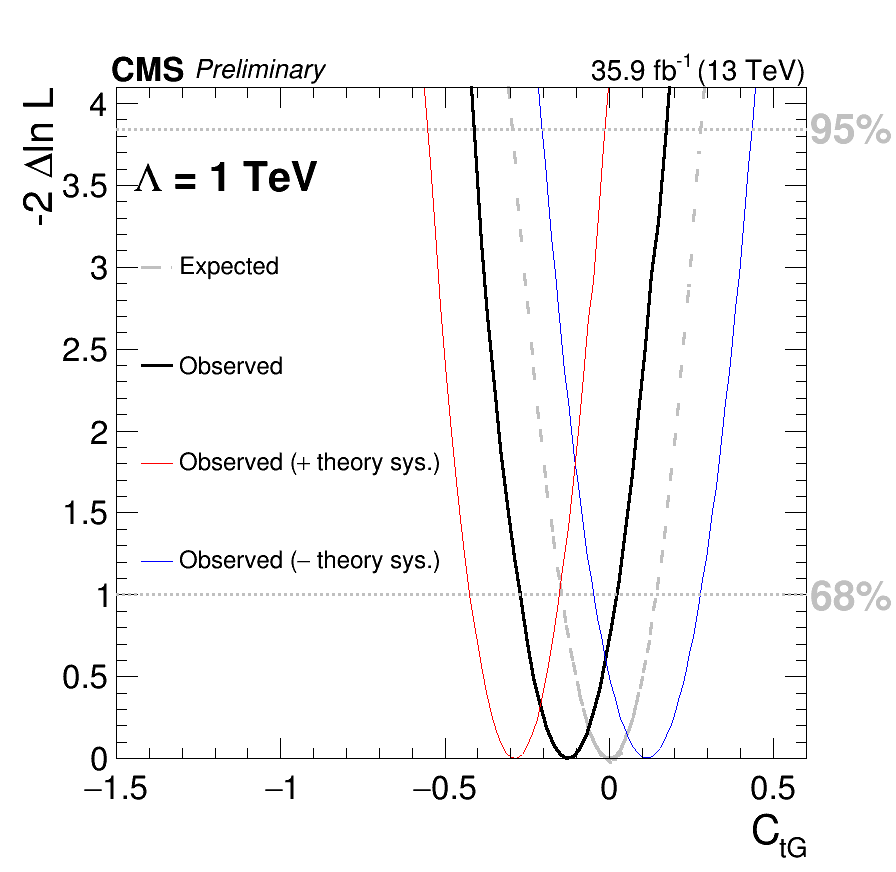
\includegraphics[width=0.45\textwidth]{figures/tW/fig/scan_all_plot/Ctg_combined_scan.png}
      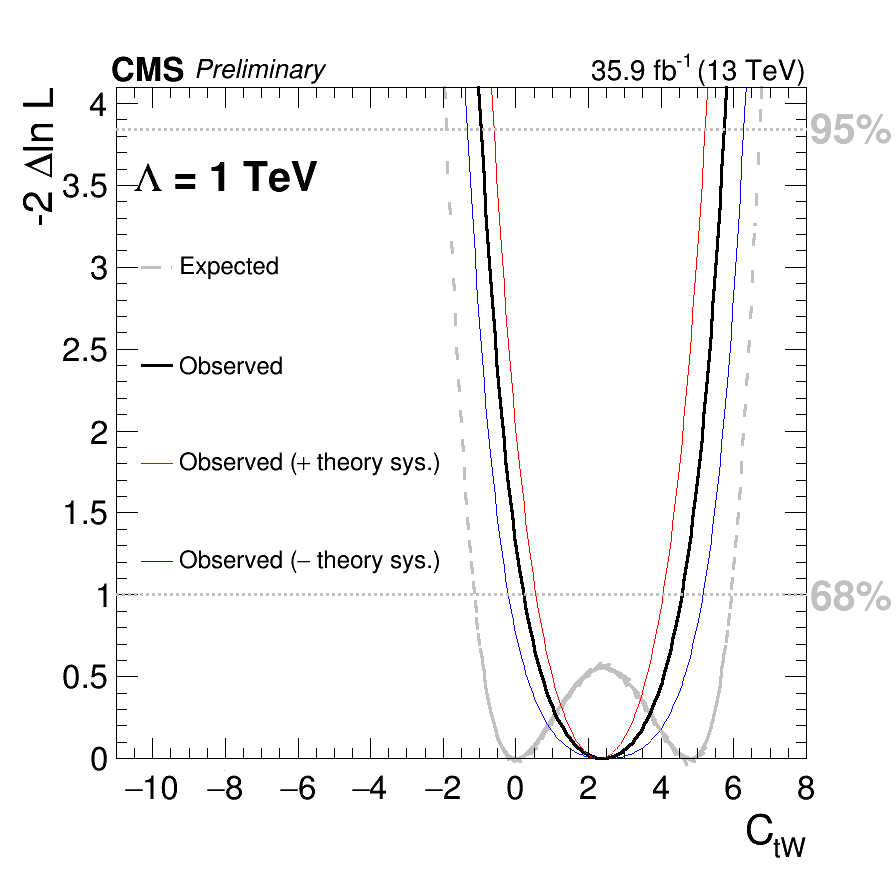
\includegraphics[width=0.45\textwidth]{figures/tW/fig/scan_all_plot/Ctw_combined_scan.png}\\
      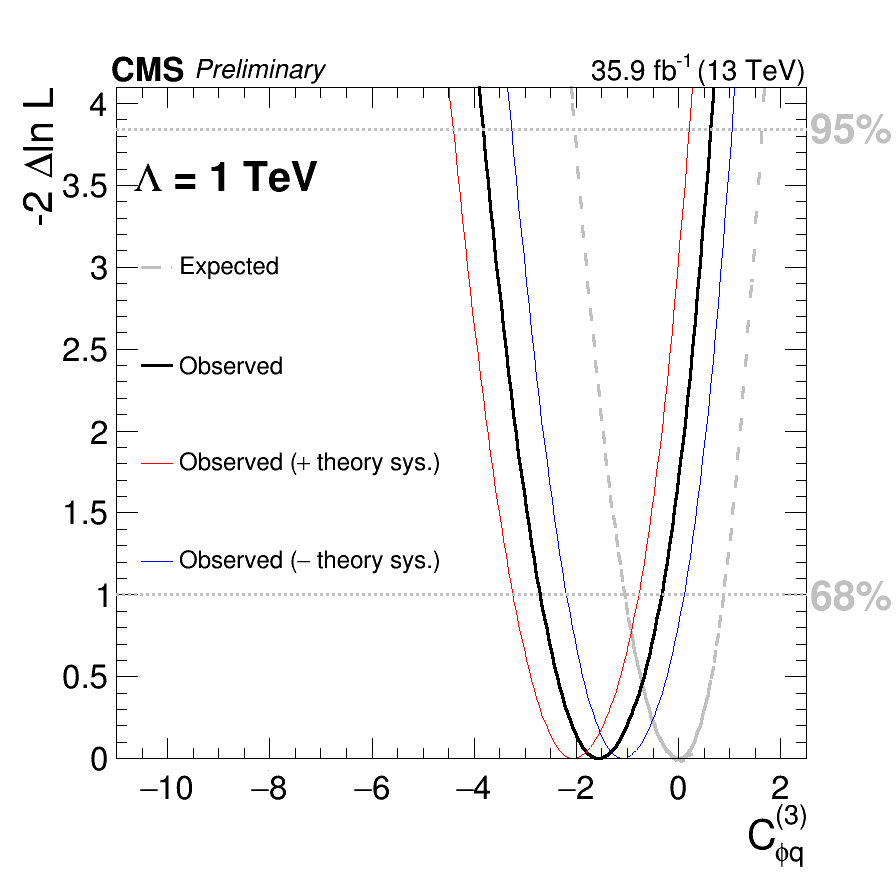
\includegraphics[width=0.45\textwidth]{figures/tW/fig/scan_all_plot/Cphiq_combined_scan.png}
    \end{tabular}
    \caption{Likelihood scans of C$_{tG}$, C$_{\phi q}$ and C$_{tW}$ effective couplings for combined channels.
    \label{fig:EFT_scan}}
  \end{center}
\end{figure}

\clearpage

\subsection {Exclusion limits on \texorpdfstring{C$_{uG}$ and C$_{cG}$  effective couplings}{}}

Since the tW production via FCNC interactions doesn't interference with the SM (with the assumption of $|\text{V}_{\text{td}}| = |\text{V}_{\text{ts}}| = 0$),
independent pdf for signal is considered  to set upper bound on related Wilson coefficients. The comparison of the MLP output for the data, SM background  and signal (tW events via FCNC interactions) in 1b-jet region are shown in Figure \ref{fig:limit_FCNC}. Here the MLP is trained to separate FCNC tW events from SM tW and \ttbar~ events as discussed in Section \ref{signal}

The limit results for individual channels and combined channels are listed in Table \ref{tab:EFT_Limit_FCNC}.
The results of the likelihood scans of the Wilson coefficients on the full 13 TeV dataset are shown in Figure \ref{fig:FCNC_scan} for combined channels.
The observed and median expected 95\% CL upper limits on the  $\sigma$(pp$\rightarrow$tW)$\times$B(W$\rightarrow \ell\nu$)$^2$ for FCNC signals are given for combined channel in Table \ref{limfcnc}.

\begin{figure}[ht]
  \begin{center}
    \begin{tabular}{ccc}
      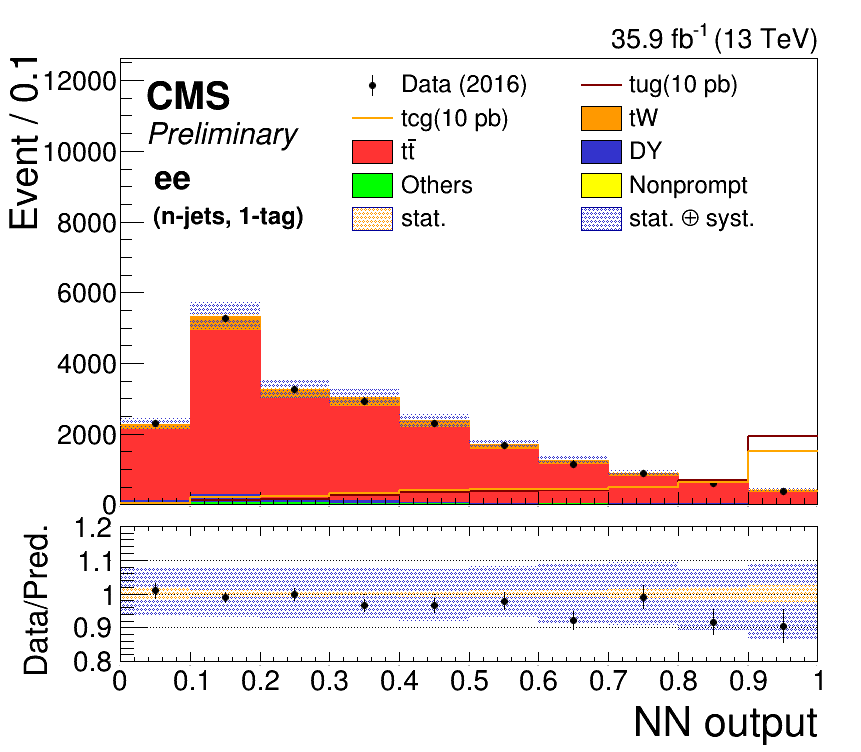
\includegraphics[width=0.45\textwidth]{figures/tW/fig/FCNC_Result/ee/H_MLP_tug_xjet_1bjet.png} &
      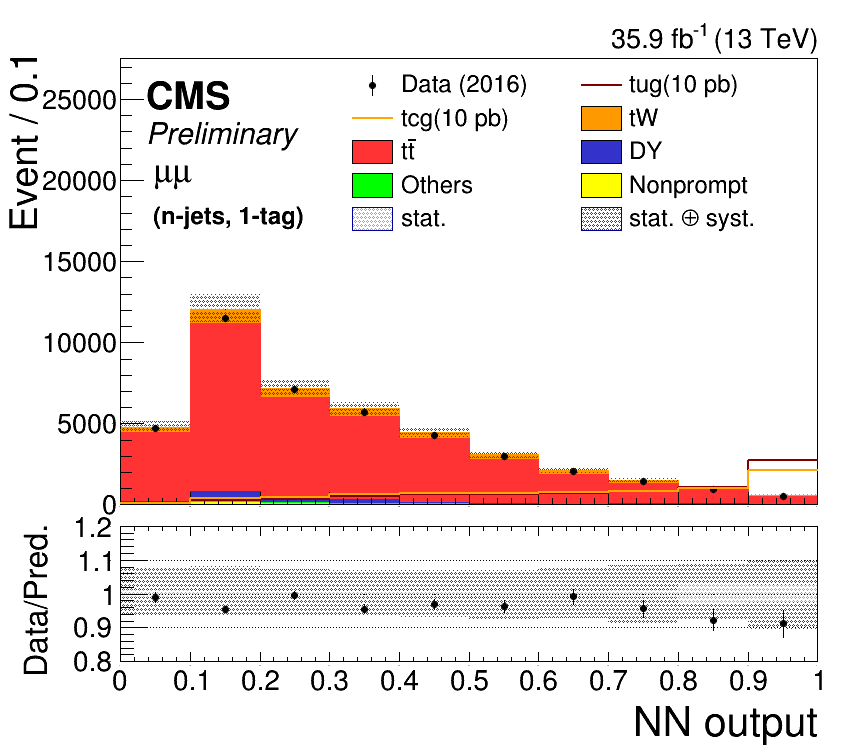
\includegraphics[width=0.45\textwidth]{figures/tW/fig/FCNC_Result/mumu/H_MLP_tug_xjet_1bjet.png}\\
    \end{tabular}
    \caption{The MLP distribution of data, MC and FCNC signals in 1b-jet region used in limit setting for $ee$ channel (left column) and $\mu\mu$ channel (right column). The blue hatched bands correspond to the sum of statistical and systematic uncertainties in the event yield for the sum of signal and background predictions. The ratios of data to the sum of the predicted yields are shown at the bottom of each plot. Here, an additional solid yellow band represents the contribution from the statistical uncertainty in the MC simulation.
    \label{fig:limit_FCNC}}
  \end{center}
\end{figure}





\begin{table}[h]
\centering
\scalebox{0.8}{
\begin{tabular}{|l|l|l|l|l|}
\hline
                               &                               & best fit exp./obs.  & 68\% exp./obs.limit                         & 95\% exp./obs.limit   \\ \hline
\multirow{4}{*}{$C_{uG}$}      & ee       NN output for (1t)   & 0.00 / -0.017& {[}-0.29 to 0.29{]}/{[}-0.224 to 0.224{]} &{[}-0.42 to 0.42{]}/{[}-0.368 to 0.368{]} \\ \cline{2-4}
                               & $\mu\mu$ NN output for (1t)   & 0.00 / -0.017& {[}-0.27 to 0.27{]}/{[}-0.167 to 0.167{]} &{[}-0.38 to 0.38{]}/{[}-0.289 to 0.289{]} \\ \cline{2-4}
                               & e$\mu$   NN output for (1t)   & 0.00 / -0.017& {[}-0.26 to 0.26{]}/{[}-0.167 to 0.167{]} &{[}-0.38 to 0.38{]}/{[}-0.290 to 0.290{]} \\ \cline{2-4}
                               & Combined                      & 0.00 / -0.017& {[}-0.21 to 0.21{]}/{[}-0.125 to 0.125{]} &{[}-0.30 to 0.30{]}/{[}-0.221 to 0.221{]} \\ \hline \hline

\multirow{4}{*}{$C_{cG}$}      & ee       NN output for (1t)   & 0.00 / -0.032& {[}-0.63 to 0.63{]}/{[}-0.471 to 0.471{]} &{[}-0.92 to 0.92{]}/{[}-0.778 to 0.778{]} \\ \cline{2-4}
                               & $\mu\mu$ NN output for (1t)   & 0.00 / -0.032& {[}-0.58 to 0.58{]}/{[}-0.363 to 0.363{]} &{[}-0.84 to 0.84{]}/{[}-0.628 to 0.628{]} \\ \cline{2-4}
                               & e$\mu$   NN output for (1t)   & 0.00 / -0.032& {[}-0.56 to 0.56{]}/{[}-0.341 to 0.341{]} &{[}-0.81 to 0.81{]}/{[}-0.599 to 0.599{]} \\ \cline{2-4}
                               & Combined                      & 0.00 / -0.032& {[}-0.46 to 0.46{]}/{[}-0.259 to 0.259{]} &{[}-0.65 to 0.65{]}/{[}-0.464 to 0.464{]} \\ \hline \hline
\end{tabular}}
\caption{Summary of allowed 68\% CL and 95\% CL intervals on C$_{uG}$ and C$_{cG}$ effective coupling  obtained in $ee$, $e\mu$, $\mu\mu$ and combined channels ($\Lambda = 1 TeV$).}
\label{tab:EFT_Limit_FCNC}
\end{table}

\begin{figure}[ht]
  \begin{center}
    \begin{tabular}{cc}
      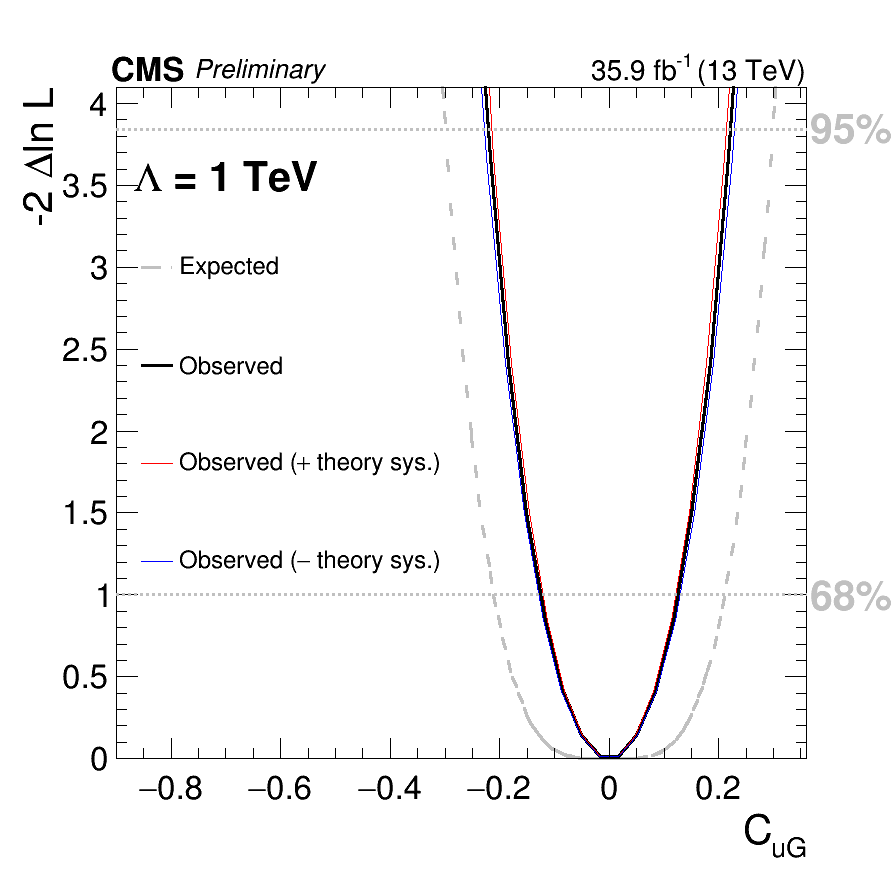
\includegraphics[width=0.45\textwidth]{figures/tW/fig/scan_all_plot/Cug_combined_scan.png}&
      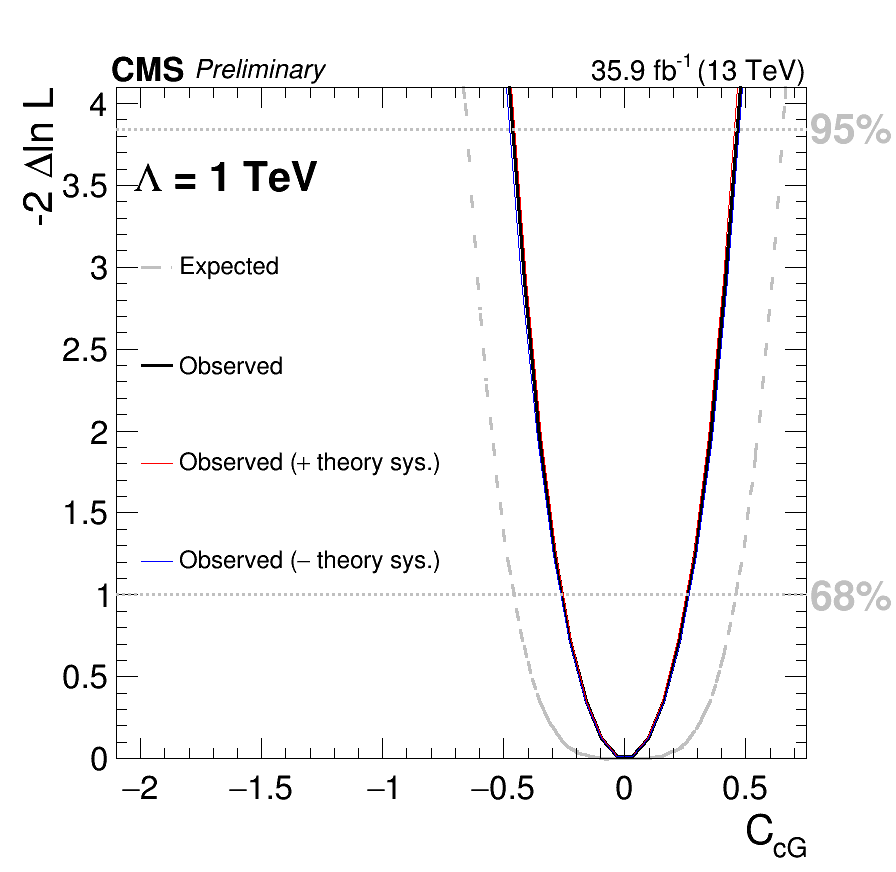
\includegraphics[width=0.45\textwidth]{figures/tW/fig/scan_all_plot/Ccg_combined_scan.png}\\
    \end{tabular}
    \caption{Likelihood scans of C$_{uG}$ and C$_{cG}$ effective couplings for combined channels.
    \label{fig:FCNC_scan}}
  \end{center}
\end{figure}

\begin{table}[h]
\centering
\begin{tabular}{|l|l|l|}
\hline
                                                                 & 68\% exp./obs.limit   & 95\% exp./obs.limit  \\ \hline
$\sigma$(pp$\rightarrow$tW)$\times$B(W$\rightarrow \ell\nu$)$^2$ &  {[}0,0.10{]}      / {[}0,0.03{]} pb  & {[}0,0.20{]}      / {[}0,0.11{]} pb   \\
$C_{uG}$($\Lambda=1$ TeV)                                        &  {[}-0.21,0.21{]}  / {[}-0.13,0.13{]} & {[}-0.30,0.30{]}  / {[}-0.22,0.22{]}  \\
B(t $\rightarrow$ ug)                                            &  {[}0,0.10918\%{]} / {[}0,0.03897\%{]}& {[}0,0.22068\%{]} / {[}0,0.12136\%{]} \\ \hline
$\sigma$(pp$\rightarrow$tW)$\times$B(W$\rightarrow \ell\nu$)$^2$ &  {[}0,0.13{]}      / {[}0,0.04{]} pb  & {[}0,0.26{]}      / {[}0,0.13{]} pb   \\
$C_{cG}$ ($\Lambda=1$ TeV)                                       &  {[}-0.46,0.46{]}  / {[}-0.26,0.26{]} & {[}-0.65,0.65{]}  / {[}-0.46,0.46{]}  \\
B(t $\rightarrow$ cg)                                            &  {[}0,0.51612\%{]} / {[}0,0.16617\%{]}& {[}0,1.05509\%{]} / {[}0,0.53367\%{]} \\ \hline
\end{tabular}
\caption{The expected and observed 95\% CL upper limits on the cross section of tW production via C$_{uG}$ and C$_{cG}$  effective couplings times square of the branching fraction B(W$\rightarrow \ell\nu$), the effective couplings C$_{uG}$ and C$_{cG}$, and the corresponding branching fractions B(t $\rightarrow$ ug) and B(t $\rightarrow$ cg).}
\label{limfcnc}
\end{table}


The expected and observed upper limits on the Wilson coefficients obtained from  the combination of all channels and signal regions are  visualized in Figure \ref{fin}.

\begin{figure}[h]
  \begin{center}
    \begin{tabular}{c}
      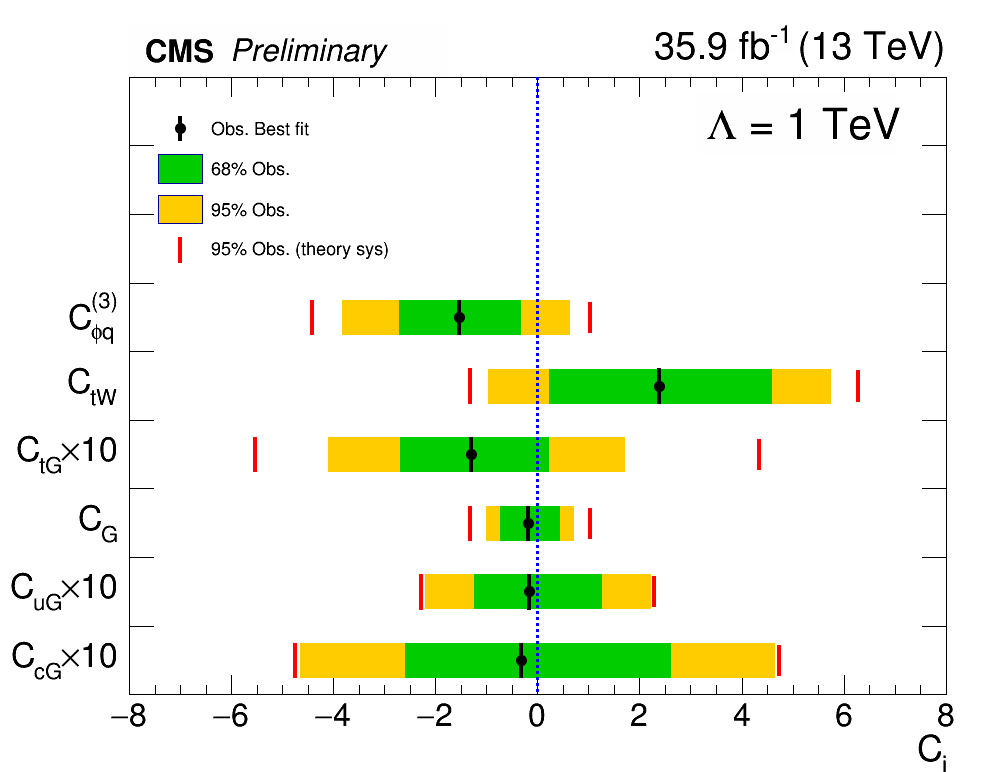
\includegraphics[width=0.9\textwidth]{figures/tW/fig/Result/tW_limit.png}\\
    \end{tabular}
    \caption{Observed and expected 95\% CL upper limits on the top quark effective couplings for combined channel ($\Lambda=1$ TeV).}
    \label{fin}
  \end{center}
\end{figure}





